% $File: design.tex
% $Date: Sat Jun 15 11:36:43 2013 +0800
% $Author: jiakai <jia.kai66@gmail.com>

\section{基本设计}
项目目录结构如下:
\dirtree{%
.1 /.
.2 hdl/\DTcomment{quartus项目文件及硬件描述代码}.
.3 src/\DTcomment{verilog源代码}.
.4 anim.v.
.4 arith.v.
.4 display.v.
.4 frame\_reader\_fh.inc.v.
.4 frame\_reader.v.
.4 frame\_reader.v.new.
.4 main.v.
.4 sigproc.v.
.3 testbench/\DTcomment{测试代码}.
.2 utils/\DTcomment{渲染及内存映象生成工具}.
.3 gen\_frame.py.
.3 gen\_mem.py.
.3 simu.py.
.2 report/\DTcomment{本报告的\LaTeX 源代码}.
.2 circuit/\DTcomment{Altium Designer工程文件}.
.2 pres/\DTcomment{基于reveal.js的presentation}.
}
以下对其中重要部分详细介绍。

\subsection{电路及PCB布局}
% f{{{
电路设计中有以下注意事项:
\begin{enumerate}
	\item Altera MAX II系列芯片可使用LM1117供电,
		它可以将3.3V至5V电压降压至3.3V,保持电源稳定。
	\item 有源晶振的电源输入、电路电源总线等需要电容滤波。
	\item 需要根据点阵的压降和电流大小,
		计算限流电阻值并在点阵和芯片输出引脚间安装限流电阻。
\end{enumerate}
整个电路的设计简单,但由于引脚多,布线较为麻烦,
还需综合考虑引脚绑定及MAX II芯片引脚分布的情况。
最初想使用4个$8\times 8$点阵,但发现布线过于困难;
后改用LM2256 $16\times 16$点阵,最终实现了在双面板上布线。
PCB的布局还需要注意对称性,以尽量平稳旋转。
电路设计详见circuit目录中的altium designer工程文件。
% f}}}

\subsection{硬件设计}
% f{{{
硬件设计的主要难点在于电路板和电动机之间的连接,
在中关村的电子城里恰好发现了比较合适的连接件,
电路板做好后通过三角挫打磨以及电钻钻孔螺丝固定,
实现了稳定可靠的连接。如下图所示:
\begin{center}
	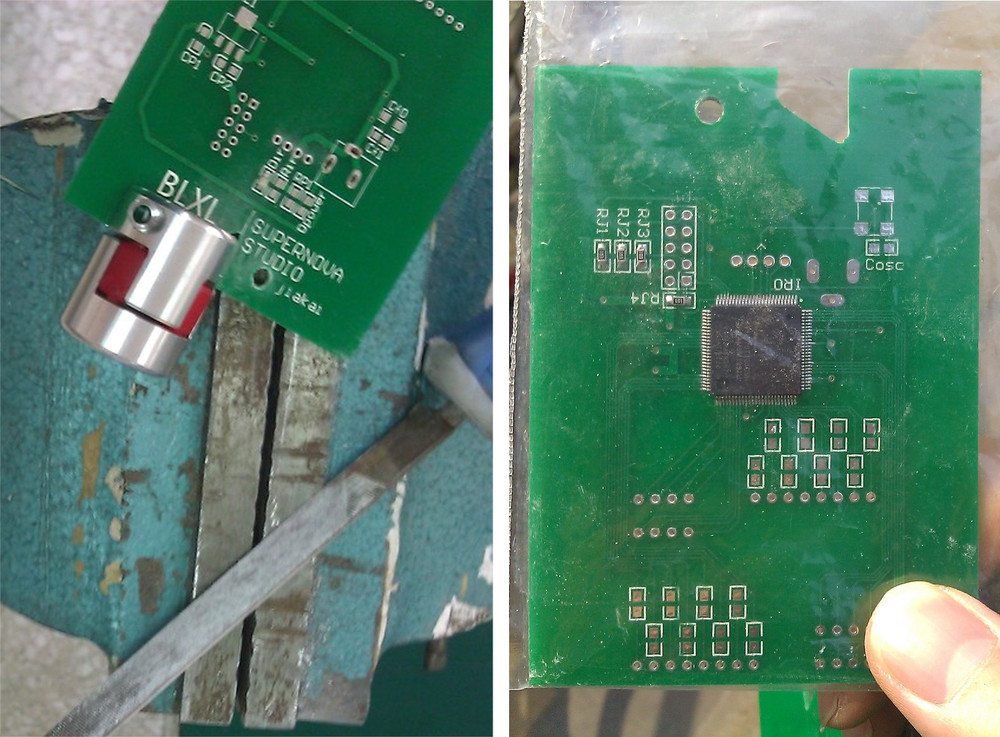
\includegraphics[width=0.5\textwidth]{../img/board_shape.jpg}
\end{center}

为了提供足够功率,使用了12V/1.5A 2000rpm的电机,
并使用电位器限流调速,以防止转速过快造成部件脱落。

在电路供电方面,曾尝试过淘宝上的无线供电模块,
测试发现输电模块发热太大,最后采取锂电池供电。

最初测试时,明显可见正前方的亮度较低,原因是LM2256自带外壳和磨砂塑料膜,
侧面观察亮度很低。曾设想在点阵表面粘贴小玻璃球以散光,实验发现效果很差;
最后设法拆掉其外壳,如下图所示,发光效果达到预期。
拆卸过程中不慎损坏了第一行第二个LED。
\begin{center}
	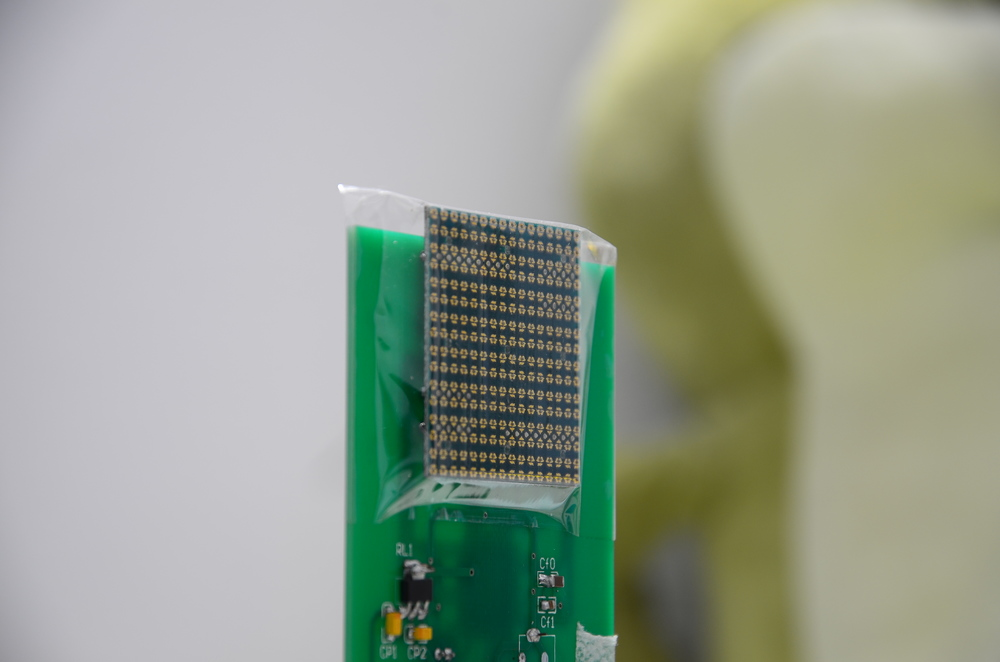
\includegraphics[width=0.6\textwidth]{../img/lm2256.jpg}
\end{center}

% f}}}

\subsection{HDL设计}
% f{{{
为了源代码的精简和可读性,放弃了VHDL而采用Verilog HDL作为硬件描述语言。

最初设想实现实时渲染,简单测试后发现EPM570的LE完全不够用,
于是考虑先软件渲染好旋转一圈中各帧的值,存入UFM,并直接播放。

基本思路是通过红外传感器,每圈得到一个信号,可得到一圈中的晶振振荡计数,
进一步求出每帧的晶振周期数,从而实现帧的切换。

\subsubsection{各文件主要功能}
\begin{enumerate}
	\item anim.v \\
		给出时钟信号及转过一圈的信号,计算当前帧编号。
	\item arith.v \\
		加一加法器及低LE用量的除法器的实现。
	\item display.v \\
		点阵像素编号到行列信号的译码。
	\item frame\_reader.v \\
		基于quartus自带的UFM SPI串行通信接口,实现UFM中给定帧编号的随机访问。
		UFM的内存布局见下文。
	\item sigproc.v \\
		信号防抖,用于处理转圈信号,
		因为实验中发现红外传感器给出的信号在跳变时貌似有短暂的不稳定。
	\item main.v \\
		描述各模块间的顶层连接。
\end{enumerate}

\subsubsection{UFM内存布局}
MAX II的UFM(User Flash Memory)能存储8192 bits,字长为16bit,故地址为9bit。
各帧要存储的内容为点亮的点的编号,由于是$16\times 16$的点阵,编号范围是0-255,
恰好8bit。最终我们在这1KiB的UFM中实现了120帧的存储。

假设要存储$N$帧,那么前$\frac{N}{2}$个word中存储各帧的首地址的低8位,
各帧首地址需要在word边缘对齐,长度为奇数的帧需添加一个冗余点以补为偶数长度。
帧首地址按帧编号递增排序,
在verilog源代码中存储了地址最高位为1的帧的最小编号$t$,
因此只用将帧编号与$t$比较就可得出其地址的第9位,再结合UFM中存储的低8位地址,
可得到各帧的完整9bit地址。用$F(k)$表示第$k$帧的首地址,
那么第$k$帧的内容位于$[F(k), F(k+1))$区间内。
% f}}}

\subsection{渲染算法及辅助工具}

将每一帧看做一个时间段,则每个像素在一帧里实际划过空间中的一个圆弧形轨迹。
软件枚举每一帧中的每一个像素,利用像素坐标、设备旋转时的偏心距以及一帧所占的圆心角,
即可计算出轨迹。
若轨迹与欲显示的空间图形的最近距离小于某阈值,则在这一帧中将此像素点亮。

实际中,规定欲显示图形只由空间线段组成。考虑一点在一圆弧上移动时,
它到给定的一条线段的距离,容易看出,这个距离要么是单调的,要么是单峰的。
因而采用三分法在圆弧上采样,就可以找到圆弧与线段的最近距离。

utils目录中gen\_frame.py用于将三维空间中的线段描述转化为各帧的值,
存储为一种帧描述文件格式;gen\_mem.py用于将帧描述转换为mif内存映象,
供quartus解析并写入UFM。simu.py则是一个基于OpenGL的3D模拟器,
读取帧描述,模拟旋转后的效果。




% vim: filetype=tex foldmethod=marker foldmarker=f{{{,f}}}

